% Options for packages loaded elsewhere
\PassOptionsToPackage{unicode}{hyperref}
\PassOptionsToPackage{hyphens}{url}
% !TeX program = pdfLaTeX
\documentclass[12pt]{article}
\usepackage{amsmath}
\usepackage{graphicx,psfrag,epsf}
\usepackage{enumerate}
\usepackage[]{natbib}
\usepackage{textcomp}


%\pdfminorversion=4
% NOTE: To produce blinded version, replace "0" with "1" below.
\newcommand{\blind}{0}

% DON'T change margins - should be 1 inch all around.
\addtolength{\oddsidemargin}{-.5in}%
\addtolength{\evensidemargin}{-1in}%
\addtolength{\textwidth}{1in}%
\addtolength{\textheight}{1.7in}%
\addtolength{\topmargin}{-1in}%

%% load any required packages here



% tightlist command for lists without linebreak
\providecommand{\tightlist}{%
  \setlength{\itemsep}{0pt}\setlength{\parskip}{0pt}}



\usepackage{booktabs}
\usepackage{longtable}
\usepackage{array}
\usepackage{multirow}
\usepackage{wrapfig}
\usepackage{float}
\usepackage{colortbl}
\usepackage{pdflscape}
\usepackage{tabu}
\usepackage{threeparttable}
\usepackage{threeparttablex}
\usepackage[normalem]{ulem}
\usepackage{makecell}
\usepackage{xcolor}

\IfFileExists{bookmark.sty}{\usepackage{bookmark}}{\usepackage{hyperref}}
\IfFileExists{xurl.sty}{\usepackage{xurl}}{} % add URL line breaks if available
\hypersetup{
  pdftitle={Climate Change and Aging: A Systematic Review},
  pdfkeywords={population aging; demography; climate impacts;
mitigation; adaptation},
  hidelinks,
  pdfcreator={LaTeX via pandoc}}



\begin{document}


\def\spacingset#1{\renewcommand{\baselinestretch}%
{#1}\small\normalsize} \spacingset{1}


%%%%%%%%%%%%%%%%%%%%%%%%%%%%%%%%%%%%%%%%%%%%%%%%%%%%%%%%%%%%%%%%%%%%%%%%%%%%%%

\if0\blind
{
  \title{\bf Climate Change and Aging: A Systematic Review}

  \author{
        Mathew E. Hauer \\
    Department of Sociology, Florida State University\\
     and \\     Kyle Rose \\
    Department of Sociology, Florida State University\\
      }
  \maketitle
} \fi

\if1\blind
{
  \bigskip
  \bigskip
  \bigskip
  \begin{center}
    {\LARGE\bf Climate Change and Aging: A Systematic Review}
  \end{center}
  \medskip
} \fi

\bigskip
\begin{abstract}
In this systematic review, we analyze the literature through Web of
Science's SCI-Expanded containing the words ``aging'' or ``aged'' and
``climate change'' and receiving at least four citations per year since
publication (n = 607 articles). After discarding irrelevant articles
(ie, ``aging infrastructure''), the 177 remaining articles
overwhelmingly (51\%) fall into two categories: temperature/mortality
(n= 67; 38\%) and temperature/morbidity (n = 24; 14\%). However, many
other important climate topics related to aging remain underdeveloped.
Notably, adaptation (n = 50; 29\%), vulnerability (n = 27; 16\%),
emissions/mitigation (n = 19; 11\%), climate perceptions (n = 13; 8\%),
drought (n = 4; 2\%), and food security (n = 2; 1\%) remain
understudied. Furthermore, more than half of the studies were conducted
in the United States (n = 46; 26\%), China (n = 0; 0\%), Globally (n =
21; 12\%), and Australia (n = 11; 6\%), suggesting a paucity of
information in the Global South (n = 11) where climate impacts will be
greatest. There were more studies specifically on Spain (n = 12) than
specifically on the entire African continent (n = 5). Finally, 27
articles (16\%) offered projections in some form, most to the middle of
the century. Gerontologists and aging scientists should look beyond the
relationship between heat and mortality to offer a more holistic view of
aging and climate change. Prospective analyses, as opposed to
retrospective, could shed additional light on the link between aging and
climate change.
\end{abstract}

\noindent%
{\it Keywords:} population aging; demography; climate impacts;
mitigation; adaptation

\vfill

\newpage
\spacingset{1.9} % DON'T change the spacing!

\hypertarget{introduction}{%
\section{Introduction}\label{introduction}}

Two seemingly immutable trends will crash head-on during this century:
the global populace will continue to age and global climate change
impacts will worsen as the century progresses. By the end of the
century, when climate change impacts will be considerably more intense
than today, the Global populace exposed to these impacts will be
decidedly older, amplifying climate change impacts. Many of the
anticipated impacts from climate change disproportionately impact older
adults versus younger, more vigorous age groups making these two trends
particularly potent when taken together.

Consider this: the Global populace will age universally. The global
population aged 75+ is expected to grow from 271M people today to nearly
1.4B people by 2100 \citep{division_wpp2017}. Today, only Japan, Italy,
and Germany have median ages in excess of 50. But by 2100, 54\% of
countries will be as old as or older than these countries are today.
These demographic trends are well known
\citep{lutz2008coming, beard2016world}.

While the global, dramatic aging shift occurs, the world will continue
to warm. Climate projections suggest global temperatures are likely
increase more than 3 degrees Celsius by 2100 compared to the
pre-industrial period \citep{arias2021climate}. These temperature
increases will likely usher in increasingly frequent and destructive
extreme weather events, more frequent droughts and wildfire risks,
extreme heat, and substantially increase the burden on health services
\citep{portner2022climate}. Low-lying coastal areas will experience
increased coastal flooding and the submergence of many coastal cities
appears likely \citep{kulp2019new}. Climate change will make the world
of 2100 considerably more precarious compared to today, a precarity
amplified by a globally aging populace.

Nearly every climate impact is heightened by age due to the older
people's social vulnerability and physiological susceptibility. Older
adults have increased social vulnerability to psychological stresses due
to environmental change, reduced ability to adapt, limited
transportation, reduced mobility, smaller social networks, lower
incomes, chronic health problems, social isolation, cognitive decline,
and general fragility \citep{kovats2008heat}. This elevated social
vulnerability combines with older adult's increased physiological
vulnerability to extreme heat and cold, extreme weather events, and
infectious diseases to create a biophysical cocktail of potential
catastrophe.

Additionally, climate change and aging intersect in multiple ways,
beyond just climate impacts. Older adults play important roles in the
mitigation or reduction of carbon emissions
\citep{oneill_global_2010, buchs_who_2013}. Adaptation to climate
impacts greatly vary among older populations
\citep{huang_is_2011, guo_high_2012} and perceptions of climate risks
can serve as barriers to effective adaptation
\citep{hansen_perceptions_2011, abrahamson_perceptions_2008}. Yet, as we
show in this article, most research concerning aging and climate change
tends to focus on the impact of extreme temperatures on older
populations. A more holistic view of the aging and climate change
literature could shed light on the varied relationships between older
adults and global environmental change.

In this article, we conduct a systematic review of the literature
surrounding climate change and aging to show two primary things. (1) We
want to show how the topic of ``climate change and population aging''
has changed over time; whether there is growing interest in the topic,
etc. (2) We want to show the primary topics where most research activity
in this area exists in order to find gaps in the research literature.

\hypertarget{methods-and-materials}{%
\section{Methods and Materials}\label{methods-and-materials}}

We use a systematic literature review to assess the literature on
climate change and aging.

\hypertarget{document-selection}{%
\subsection{Document selection}\label{document-selection}}

We used a keyword search on Clarivate's Web of Science-expanded search
engine using the Boolean operator ``TS=(aging OR aged OR elderly) AND
TS=(``climate change'').'' We selected Web of Science due to its
comprehensive scientific coverage of peer-reviewed literature. We
conducted the search on September 7, 2022. This search retrieved an
initial universe of 16,828 articles. We filtered these results to
include articles of relatively high impact, defined subjectively as
those articles with at least four citations per year (n = 3,852). To
further isolate those articles pertaining to aging and climate change,
we further restricted our search to those articles containing the words
(aging or aged or elderly) in the abstract (n = 607).

We then reviewed these articles for relevance, discarding articles
concerning ``aging infrastructure'' or ``aging forests'' to isolate
articles on human aging and climate change. This yielded a total of 177
articles included in this systematic review
(\textbf{\autoref{fig-diagram}}).

\begin{figure}
\centering
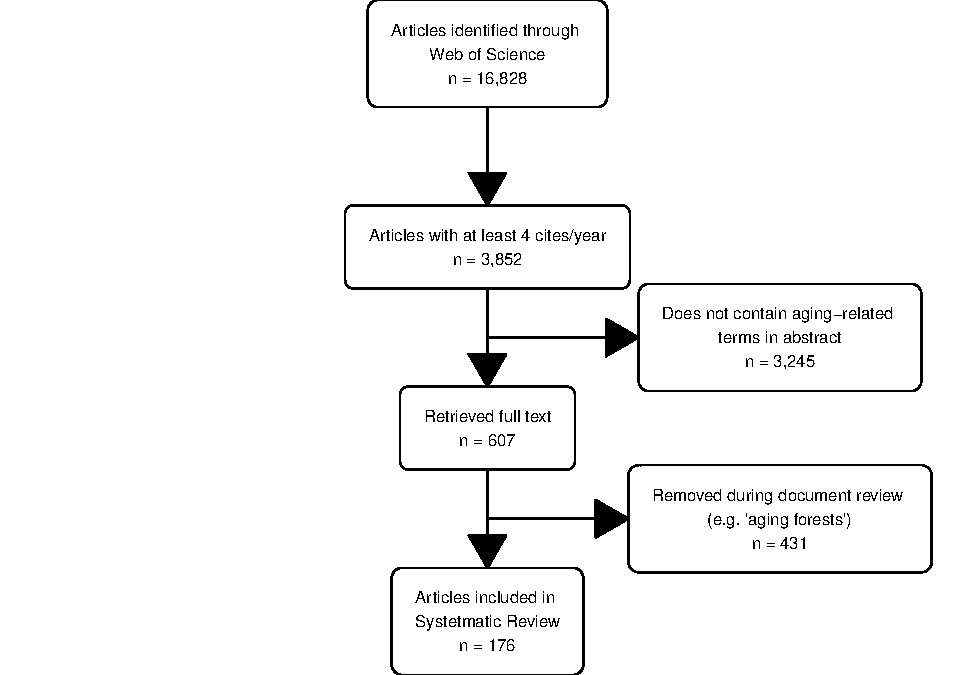
\includegraphics{MainDocument_files/figure-latex/figureflowdiagram-1.pdf}
\caption{PRISMA Flow Diagram. \label{fig-diagram}}
\end{figure}

\hypertarget{document-review}{%
\subsection{Document review}\label{document-review}}

Following our document selection and screening, 607 articles were
retained for full review. We developed a questionnaire to survey these
articles to document and characterize the primary topics of climate
change. We developed this questionnaire to standardize the analysis,
produce descriptive statistics, and examine trends. We coded all papers
based on:

\begin{enumerate}
\def\labelenumi{(\arabic{enumi})}
\tightlist
\item
  the primary and (2) secondary climate effect studied,
\item
  the climate impact type (sensitivity, vulnerability, or exposure),
\item
  the climate impact studied (morbidity, mortality, etc.), if the
  article concerned
\item
  mitigation, (6) adaptation, or (7) perceptions,
\item
  if the article included a projection,
\item
  the historic time period, and
\item
  the general area the study was conducted.
\end{enumerate}

Additionally, we gathered general information on authorship, publication
year, and citation counts. We conducted an extensive full-text review of
all (n = 607) articles using this questionnaire. We assessed the primary
finding in articles where multiple climate impact types or climate
impacts were studied.

\hypertarget{analysis}{%
\subsection{Analysis}\label{analysis}}

All (n = 16,828) articles were retained for validation. All data were
entered into an Excel spreadsheet. We used R to analyze the data and to
produce descriptive statistics and visualizations.

\hypertarget{data-availability}{%
\section{Data Availability}\label{data-availability}}

The underlying computer code and data that support the findings of this
study are available in the Supplementary Material and have been
deposited in Zenodo (DOI).

\hypertarget{results}{%
\section{Results}\label{results}}

\hypertarget{general-interest-in-aging-and-climate-change}{%
\subsection{General Interest in Aging and Climate
Change}\label{general-interest-in-aging-and-climate-change}}

\textbf{\autoref{fig-timelines}} shows the trends in articles
(\textbf{\autoref{fig-timelines}a}), cumulative citations
(\textbf{\autoref{fig-timelines}b}), and average citations per year
(\textbf{\autoref{fig-timelines}c}) for our compendium on `climate
change and aging.' Our compendium shows that the number of articles has
been steadily increasing since 2000, peaking in 2019, most likely due to
the exclusion criteria of four citations per year. However, the total
number of citations in our database peaks much earlier in 2010. This
peak roughly coincides with the publication of the IPCC's AR4 report in
2007 and with several publications documenting heat mortality associated
with the 2003 European summer heatwaves. The increasing number of
published articles per year is encouraging but it is discouraging that
the more recent literature is likely having less impact than the older
literature in this area.

\begin{figure}
\centering
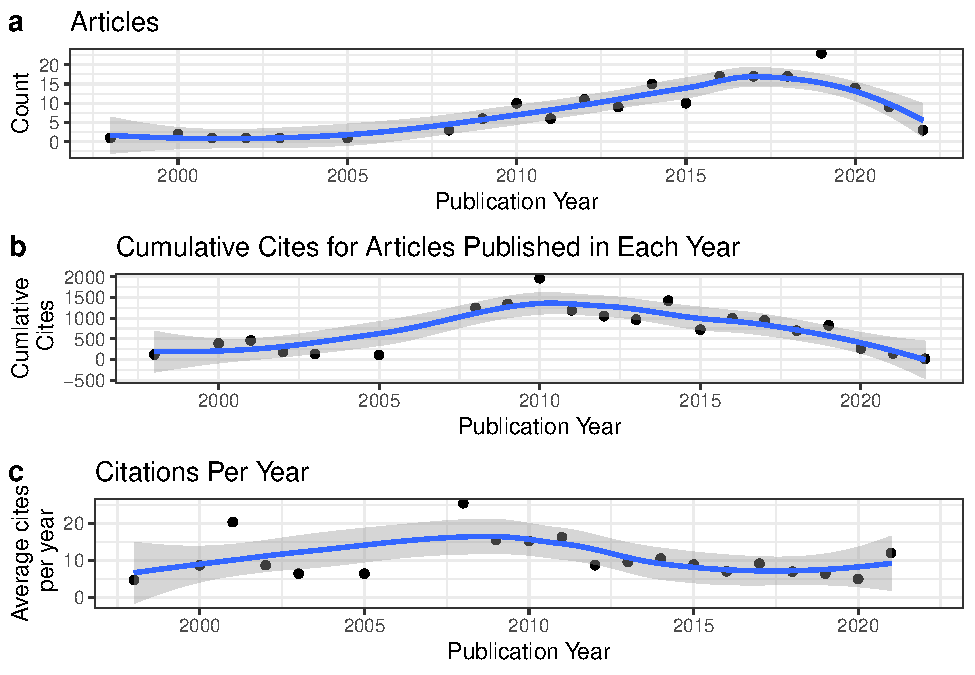
\includegraphics{MainDocument_files/figure-latex/mapandtimelines-1.pdf}
\caption{\textbf{Published articles, cumulative citations, and citations per year since 1998 for 'aging' and 'climate change' articles reviewed.}
(a) shows the number of articles published each year, (b) shows the
cumulative citations for articles published in each year, and (c) shows
the citations per article per year. Articles published have increased
since 1998, but there has been a small decline in this literature since
2020. The most cited articles and the citations per year per article
peaked more than 10 years ago, possibly suggesting a waning interest in
this literature. \label{fig-timelines}}
\end{figure}

\hypertarget{population-aging-and-climate-effects-and-impacts}{%
\subsection{Population Aging and Climate Effects and
Impacts}\label{population-aging-and-climate-effects-and-impacts}}

\textbf{\autoref{fig-heatmap}} illustrates the co-occurrences of climate
effects and climate impacts. The overwhelming majority of articles in
our sample concerned temperature as a climate effect (n = 98). Some
examples of climate effects which were classified as temperature include
heat (n = 29), heatwaves (n = 18), daily temperature range (n = 9) and
ambient temperature (n = 8).

The large majority of articles in our sample concerned the climate
impact on mortality (n =81) and morbidity (n = 31). The morbidity
category included articles which specifically observe ``morbidity'' (n =
22), hospital admissions (n = 8) and ambulance attendance (n = 1), among
others.

More than half of the articles in our sample which included climate
effects were specifically about the impact of temperature on mortality
(n = 88). The second most frequent climate effect and impact to be
studied together was temperature and morbidity (n = 35). The studies in
our sample overwhelmingly find that higher temperatures are associated
with elevated mortality and morbidity among older populations. Our
findings suggest that the most popular climate change features studied
in relation to aging populations are temperature effects like heat index
and temperature variability on morbidity and mortality metrics like
hospital attendance or years of life lost.

There is also a small section of literature which concerns the effect of
pollution on aging populations (n = 17). Two-thirds of these articles,
like temperature, concerned pollution's impact on either mortality (n =
6) or morbidity (n = 2).

There is a paucity of information on how droughts, extreme weather, and
sea-level rise (SLR) will impact aging human populations. Cumulatively,
12 articles observed any of these effects of climate change.
Specifically, we find that pollution, flooding and SLR, extreme weather
and wildfires, and drought are understudied in the literature. Climate
impacts are incredibly varied in the broader climate change literature
but \emph{not} in the climate change and aging literature.

Importantly, very few articles observe the relationships between the
broader set of climate effects and human behaviors, such as migration,
economic activity, and climate behaviors \& policies (n = 3). Only
studies examining morbidity and mortality concerned multiple climate
impacts. This gap is particularly pressing because it speaks to aging
populations' abilities to respond to climate change. It is conceivable
that aging populations may respond to sea-level rise with migration,
urban heat islands with outdoor green spaces, extreme weather events
with improved household infrastructure, or seasonal temperature
variation with voting behavior. All of these examples demonstrate how
climate effects can impact human behavior and, consequently, adaptive
capacity among older populations, yet all remain understudied.

\begin{figure}
\centering
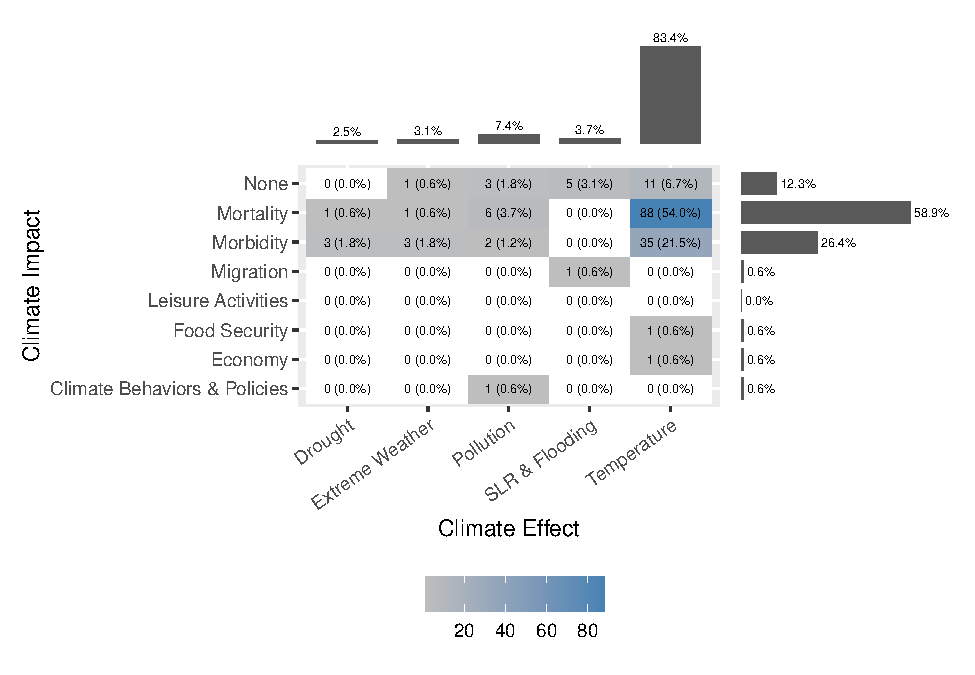
\includegraphics{MainDocument_files/figure-latex/heatmapcrosstab-1.pdf}
\caption{\textbf{Heatmap of Common Characteristics.} Here we show the
commonalities in the papers we reviewed. The numbers in each square show
both the number and relative frequency of the joint climat
impact/effect. Most articles on `Aging and Climate Change' concern the
relationship between temperature and mortality (86 articles or 54\%) or
temperature and morbidity (35 articles or 21.5\%). Very few studies
touch on other climate impacts such as drought or Extreme weather. Those
categorized with no climate impact often investigated exposure or
vulnerability, broadly defined. \label{fig-heatmap}}
\end{figure}

\hypertarget{older-adults-vulnerability-to-climate-change}{%
\subsection{Older Adults' Vulnerability to Climate
Change}\label{older-adults-vulnerability-to-climate-change}}

\textbf{\autoref{table-vesa}} reports broad categories of the components
of vulnerability. Vulnerability is often given as the function
\(V=E\cdot S \cdot A\), where Vulnerability is equal to the product of
Exposure to a climate hazard, Sensitivity to a given climate hazard, and
Adaptive capacity \citep{field2014climate, parmesan2022climate}.
However, the scientific literature surrounding population aging and
climate change overwhelmingly studies vulnerability as a function of
exposure (n=51) and sensitivity (n=89), with very few studies on
vulnerability concerning adaptive capacity (n=8). Furthermore, only ten
articles in our sample analyzed vulnerability with the complete
complement of VESA. Adaptation potential and gaps among older
populations are seriously understudied in the broader literature.

\begin{table}[]
\centering
\resizebox{\textwidth}{!}{\begin{tabular}{lllll|l}
                                                & \textbf{Vulnerability} & \textbf{Exposure} & \textbf{Sensitivity} & \textbf{Adaptive Capacity} & \textbf{TOTAL} \\ \cline{2-6} 
\multicolumn{1}{l|}{\textbf{Vulnerability}}     & 25                     & 4                 & 11                   & 0                          & 40             \\
\multicolumn{1}{l|}{\textbf{Exposure}}          & 4                      & 6                 & 39                   & 2                          & 51             \\
\multicolumn{1}{l|}{\textbf{Sensitivity}}       & 11                     & 39                & 38                   & 1                          & 89             \\
\multicolumn{1}{l|}{\textbf{Adaptive Capacity}} & 0                      & 2                 & 1                    & 5                          & 8              \\ \hline
\end{tabular}}
\caption{\textbf{Number of articles broadly categorized as aspects of Vulnerability.} Vulnerability is often defined as VESA, where Vulnerability is equal to exposure multiplied by sensitivity multiplied by adaptive capacity. Most published research on climate change and population aging focuses on sensitivity and exposure while very little published researches concerns adaptive capacity. A large number of articles (n=40) use an amphorous definition of `vulnerability.'}\label{table-vesa} 
\end{table}

\hypertarget{aging-and-climate-change-among-broader-climate-change-categories}{%
\subsection{Aging and Climate Change among Broader Climate Change
Categories}\label{aging-and-climate-change-among-broader-climate-change-categories}}

\textbf{\autoref{table-broad}} shows the number of journal articles
categorized into broad climate categories to show additional gaps in the
climate change and population aging literature. The IPCC is split into
three working groups, two of which are highly relevant to population
aging: Impacts/Adaptation/Vulnerability and Mitigation. Less than
one-third of articles (n=51) had any form of adaptation to climate
change, slightly more than 10\% of articles concerned mitigating carbon
emissions, and just 7\% of articles contained any form of research on
perceptions of climate change. Most articles concern some form of
climate impact (\textbf{\autoref{fig-heatmap}}) but considerably fewer
articles concern adaptation to climate change for older adults. Most
articles contained some form of retrospective analysis (n=118) but few
studies carried that retrospective analysis into a prospective analysis
(n=27) or demonstrating a gap in how future climate change could impact
future older adults.

Additionally, mitigating carbon emissions are a key mission of the IPCC
to ensure our planet remains habitable in the long term. Unfortunately,
few articles (n=13) concern any form of mitigation of carbon emissions
among older adults, suggesting a very sizable research gap.

\begin{table}[]
\centering
\begin{tabular}{llll}
              & Yes & No  & \%   \\ \hline
Adaptation    & 51  & 126 & 29\% \\
Mitigation    & 19  & 158 & 11\% \\
Perceptions   & 13  & 164 & 7\%  \\ \hline
Retrospective & 118 & 59  & 67\% \\
Prospective   & 27  & 149 & 15\% \\ \hline
\end{tabular}
\caption{\textbf{Number of articles broadly categorized as aspects of climate change research.} The IPCC is split into three working groups: the physical science, Impacts/Adaptation/Vulnerability, and Mitigation. The scientific literature concerning population aging and climate change has many articles on Impacts, few on adaptation, and a paucity on mitigation. Additionally, perceptions of climate change is also considerably understudied. Finally, we categorized articles that contained retrospective and prospective analyses. Most articles contained a historical analysis but few concerned some form of projected impact (n=27).}\label{table-broad} 
\end{table}

\hypertarget{the-geography-of-the-literature}{%
\subsection{The Geography of the
Literature}\label{the-geography-of-the-literature}}

\begin{figure}
\centering
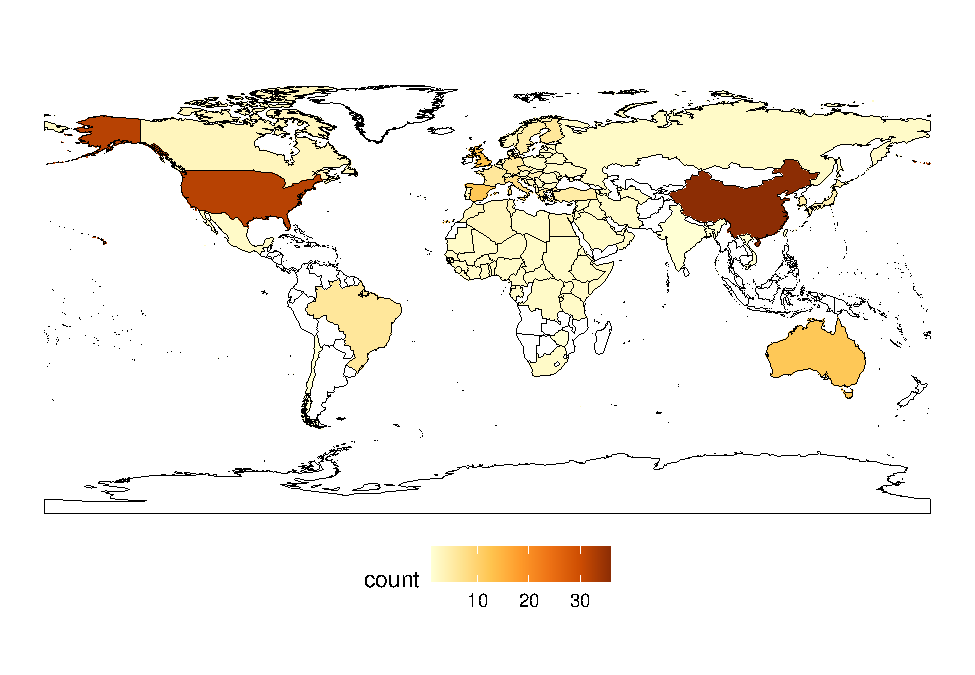
\includegraphics{MainDocument_files/figure-latex/map-1.pdf}
\caption{\textbf{Map of where studies were carried out.} Here we show
the geographic locations of where studies were conducted. Most studies
on aging and climate change were conducted in the global north, where
most of the current older populations reside rather in the global south,
where most of the climate impacts will occur. \label{fig-map}}
\end{figure}

We also gathered information on the countries on which studies were
conducted. \textbf{\autoref{fig-map}} shows the geographic location of
where studies were conducted. Geographically, the literature on aging
and climate change could use a lot of work, to put it charitably. China
(n= 36), the USA (n=32), and Global (n=21) account for half of the
literature. African countries, the average African country has just two
studies, South America, dominated by studies on Brazil (n=6), and
Southeast Asia, where Vietnam has just a single study, are regions of
the world that are still massively understudied in this literature.

The regions most impacted by climate change, but also with the most
youthful populations, are the most understudied. And the regions least
impacted by climate change, but with the most older populations, are the
most studied. There were more studies specifically on Spain (n = 12)
than specifically on the entire African continent (n = 5).

\hypertarget{conclusion}{%
\section{Conclusion}\label{conclusion}}

In this article, we conducted a systematic literature review of
``population aging'' and ``climate change'' to identify the primary
topics of research activity. We found that the majority of articles
concerned temperature and mortality or temperature and morbidity,
finding that older adults are particularly susceptible to extreme
temperatures. Climate change impacts go far beyond just temperature yet
the literature surrounding these impacts for older adults remain
severely underdeveloped. We also show that most studies are conducted in
the global north, where presently most of the world's older population
resides. Conversely, few studies are conducted in the global south, the
locations with the most severe climate impacts.

Based on our analysis we have several recommendations for scientists
working at the intersection of population aging and climate change.
First, we suggest that scientists broaden their analyses of climate
impacts beyond temperature. The IPCC Assessment Report 6 lists a number
of climate impacts beyond temperature that include food security, water
security, malnutrition, food safety, vector-borne diseases, heavy
precipitation events and flooding, migration and displacement, loss of
income and livelihoods, international armed conflict, sea-level rise,
and economic damages, to name just a few. How these climate impacts will
effect older populations is still poorly understood. Scientists would do
well to focus on a broader set of climate impacts to better holistically
understand how climate change will impact older populations.

Second, we suggest that scientists working at the intersection of
climate change and aging broaden their scope of vulnerability. In
particular, the literature surrounding older populations' adaptive
capacity is severely limited compared to exposure and sensitivity. The
extent to which older adults have the capacity to adapt to climate
change and their ability to adapt are still understudied. We know that
climate change will change the extent of exposure to climate harms and
we largely know that older adults are particularly susceptible to
climate impacts. However, the capabilities of older adults to adapt to
climate change is still too unknown.

Third, we suggest that scientists focus additional research in the
regions that will experience the greatest impacts from climate change.
Our understanding of climate change and older adults is still too
focused on the developed, global north, where climate impacts are the
least intense. We know comparatively very little about how older
populations in less developed, global south countries will be impacted
by climate change. This is a particularly pernicious gap in the
literature since these areas will be impacted the most.

Fourth, mitigation of carbon emissions is a key component to ensure we
avoid the most damages from climate change. Yet studies on mitigation
among older adults are still a small fraction of this literature. As the
global population continues to age, mitigation strategies among older
adults will become increasingly important and should receive additional
focus from scientists. If we are to develop effective mitigation
strategies, older adults will become an increasingly important
population.

Fifth, and finally, climate change and older adults goes far beyond
climate impacts, adaptive capacity, geography, and mitigation. We
reviewed not a single article on older adults and climate denial, for
instance. By largely limiting our understanding of climate change to the
mortality and morbidity of older adults during extreme temperatures,
scientists are missing important topics in climate change such as
transitions to net-zero carbon emissions, climate denial, resilience,
planned relocation, and inequality. Successfully tackling the climate
crisis will require broader conceptualizations of ``climate change'' and
``aging'' than presently found in the scientific literature.

\hypertarget{appendix---articles-included-in-review}{%
\section{Appendix - Articles Included in
Review}\label{appendix---articles-included-in-review}}

Abrahamson, V., J. Wolf, I. Lorenzoni, B. Fenn, S. Kovats, P. Wilkinson,
W. N. Adger, and R. Raine. 2008. ``Perceptions of Heatwave Risks to
Health: Interview-Based Study of Older People in London and Norwich,
UK.'' Journal of Public Health 31(1):119--26. doi:
10.1093/pubmed/fdn102.

Achakulwisut, P., L. J. Mickley, and S. C. Anenberg. 2018.
``Drought-Sensitivity of Fine Dust in the US Southwest: Implications for
Air Quality and Public Health under Future Climate Change.''
Environmental Research Letters 13(5):054025. doi:
10.1088/1748-9326/aabf20.

Achebak, Hicham, Daniel Devolder, and Joan Ballester. 2019. ``Trends in
Temperature-Related Age-Specific and Sex-Specific Mortality from
Cardiovascular Diseases in Spain: A National Time-Series Analysis.'' The
Lancet Planetary Health 3(7):e297--306. doi:
10.1016/S2542-5196(19)30090-7.

Ahmadalipour, Ali, and Hamid Moradkhani. 2018. ``Escalating Heat-Stress
Mortality Risk Due to Global Warming in the Middle East and North Africa
(MENA).'' Environment International 117:215--25. doi:
10.1016/j.envint.2018.05.014.

Ahmadalipour, Ali, Hamid Moradkhani, and Mukesh Kumar. 2019. ``Mortality
Risk from Heat Stress Expected to Hit Poorest Nations the Hardest.''
Climatic Change 152(3--4):569--79. doi: 10.1007/s10584-018-2348-2.

Anderson, G. Brooke, Francesca Dominici, Yun Wang, Meredith C.
McCormack, Michelle L. Bell, and Roger D. Peng. 2013. ``Heat-Related
Emergency Hospitalizations for Respiratory Diseases in the Medicare
Population.'' American Journal of Respiratory and Critical Care Medicine
187(10):1098--1103. doi: 10.1164/rccm.201211-1969OC.

Andrade, Maria de Fatima, Prashant Kumar, Edmilson Dias de Freitas, Rita
Yuri Ynoue, Jorge Martins, Leila D. Martins, Thiago Nogueira, Pedro
Perez-Martinez, Regina Maura de Miranda, Taciana Albuquerque, Fabio Luiz
Teixeira Gonçalves, Beatriz Oyama, and Yang Zhang. 2017. ``Air Quality
in the Megacity of São Paulo: Evolution over the Last 30 Years and
Future Perspectives.'' Atmospheric Environment 159:66--82. doi:
10.1016/j.atmosenv.2017.03.051.

Arbuthnott, Katherine G., and Shakoor Hajat. 2017. ``The Health Effects
of Hotter Summers and Heat Waves in the Population of the United
Kingdom: A Review of the Evidence.'' Environmental Health 16(S1):119.
doi: 10.1186/s12940-017-0322-5.

Baquero Larriva, María Teresa, and Ester Higueras. 2020. ``Health Risk
for Older Adults in Madrid, by Outdoor Thermal and Acoustic Comfort.''
Urban Climate 34:100724. doi: 10.1016/j.uclim.2020.100724.

Bassil, Kate, and Donald Cole. 2010. ``Effectiveness of Public Health
Interventions in Reducing Morbidity and Mortality during Heat Episodes:
A Structured Review.'' International Journal of Environmental Research
and Public Health 7(3):991--1001. doi: 10.3390/ijerph7030991.

Bell, Michelle L., Marie S. O'Neill, Nalini Ranjit, Victor H.
Borja-Aburto, Luis A. Cifuentes, and Nelson C. Gouveia. 2008.
``Vulnerability to Heat-Related Mortality in Latin America: A
Case-Crossover Study in São Paulo, Brazil, Santiago, Chile and Mexico
City, Mexico.'' International Journal of Epidemiology 37(4):796--804.
doi: 10.1093/ije/dyn094.

Benevolenza, Mia A., and LeaAnne DeRigne. 2019. ``The Impact of Climate
Change and Natural Disasters on Vulnerable Populations: A Systematic
Review of Literature.'' Journal of Human Behavior in the Social
Environment 29(2):266--81. doi: 10.1080/10911359.2018.1527739.

Benmarhnia, Tarik, Zinzi Bailey, David Kaiser, Nathalie Auger, Nicholas
King, and Jay S. Kaufman. 2016. ``A Difference-in-Differences Approach
to Assess the Effect of a Heat Action Plan on Heat-Related Mortality,
and Differences in Effectiveness According to Sex, Age, and
Socioeconomic Status (Montreal, Quebec).'' Environmental Health
Perspectives 124(11):1694--99. doi: 10.1289/EHP203.

Benmarhnia, Tarik, Wahida Kihal-Talantikite, Martina S. Ragettli, and
Séverine Deguen. 2017. ``Small-Area Spatiotemporal Analysis of Heatwave
Impacts on Elderly Mortality in Paris: A Cluster Analysis Approach.''
Science of The Total Environment 592:288--94. doi:
10.1016/j.scitotenv.2017.03.102.

Berman, Jesse D., Keita Ebisu, Roger D. Peng, Francesca Dominici, and
Michelle L. Bell. 2017. ``Drought and the Risk of Hospital Admissions
and Mortality in Older Adults in Western USA from 2000 to 2013: A
Retrospective Study.'' The Lancet Planetary Health 1(1):e17--25. doi:
10.1016/S2542-5196(17)30002-5.

Berrang-Ford, Lea, James D. Ford, and Jaclyn Paterson. 2011. ``Are We
Adapting to Climate Change?'' Global Environmental Change 21(1):25--33.
doi: 10.1016/j.gloenvcha.2010.09.012.

Bobb, Jennifer F., Ziad Obermeyer, Yun Wang, and Francesca Dominici.
2014. ``Cause-Specific Risk of Hospital Admission Related to Extreme
Heat in Older Adults.'' JAMA 312(24):2659. doi: 10.1001/jama.2014.15715.

Borchers Arriagada, Nicolas, David M. J. S. Bowman, Andrew J. Palmer,
and Fay H. Johnston. 2020. ``Climate Change, Wildfires, Heatwaves and
Health Impacts in Australia.'' Pp. 99--116 in Extreme Weather Events and
Human Health, edited by R. Akhtar. Cham: Springer International
Publishing.

Büchs, Milena, and Sylke V. Schnepf. 2013. ``Who Emits Most?
Associations between Socio-Economic Factors and UK Households' Home
Energy, Transport, Indirect and Total CO2 Emissions.'' Ecological
Economics 90:114--23. doi: 10.1016/j.ecolecon.2013.03.007.

Bunker, Aditi, Jan Wildenhain, Alina Vandenbergh, Nicholas Henschke,
Joacim Rocklöv, Shakoor Hajat, and Rainer Sauerborn. 2016. ``Effects of
Air Temperature on Climate-Sensitive Mortality and Morbidity Outcomes in
the Elderly; a Systematic Review and Meta-Analysis of Epidemiological
Evidence.'' EBioMedicine 6:258--68. doi: 10.1016/j.ebiom.2016.02.034.

Burkart, Katrin, Susanne Breitner, Alexandra Schneider, Md. Mobarak
Hossain Khan, Alexander Krämer, and Wilfried Endlicher. 2014. ``An
Analysis of Heat Effects in Different Subpopulations of Bangladesh.''
International Journal of Biometeorology 58(2):227--37. doi:
10.1007/s00484-013-0668-5.

Burkett, Ellen, Melinda G. Martin-Khan, Justin Scott, Mayukh Samanta,
and Leonard C. Gray. 2017. ``Trends and Predicted Trends in
Presentations of Older People to Australian Emergency Departments:
Effects of Demand Growth, Population Aging and Climate Change.''
Australian Health Review 41(3):246. doi: 10.1071/AH15165.

Bustinza, Ray, Germain Lebel, Pierre Gosselin, Diane Bélanger, and Fateh
Chebana. 2013. ``Health Impacts of the July 2010 Heat Wave in Québec,
Canada.'' BMC Public Health 13(1):56. doi: 10.1186/1471-2458-13-56.

Calleja-Agius, Jean, Kathleen England, and Neville Calleja. 2021. ``The
Effect of Global Warming on Mortality.'' Early Human Development
155:105222. doi: 10.1016/j.earlhumdev.2020.105222.

Carter, Timothy R., Stefan Fronzek, Aino Inkinen, Ismo Lahtinen, Matti
Lahtinen, Hanna Mela, Karen L. O'Brien, Lynn D. Rosentrater, Reija
Ruuhela, Louise Simonsson, and Emma Terama. 2016. ``Characterising
Vulnerability of the Elderly to Climate Change in the Nordic Region.''
Regional Environmental Change 16(1):43--58. doi:
10.1007/s10113-014-0688-7.

Chambers, Jonathan. 2020. ``Global and Cross-Country Analysis of
Exposure of Vulnerable Populations to Heatwaves from 1980 to 2018.''
Climatic Change 163(1):539--58. doi: 10.1007/s10584-020-02884-2.

Chen, Kai, Arlene M. Fiore, Renjie Chen, Leiwen Jiang, Bryan Jones,
Alexandra Schneider, Annette Peters, Jun Bi, Haidong Kan, and Patrick L.
Kinney. 2018. ``Future Ozone-Related Acute Excess Mortality under
Climate and Population Change Scenarios in China: A Modeling Study''
edited by J. Patz. PLOS Medicine 15(7):e1002598. doi:
10.1371/journal.pmed.1002598.

Chen, Kai, Ana Maria Vicedo-Cabrera, and Robert Dubrow. 2020.
``Projections of Ambient Temperature- and Air Pollution-Related
Mortality Burden Under Combined Climate Change and Population Aging
Scenarios: A Review.'' Current Environmental Health Reports
7(3):243--55. doi: 10.1007/s40572-020-00281-6.

Chen, Kai, Lian Zhou, Xiaodong Chen, Zongwei Ma, Yang Liu, Lei Huang,
Jun Bi, and Patrick L. Kinney. 2016. ``Urbanization Level and
Vulnerability to Heat-Related Mortality in Jiangsu Province, China.''
Environmental Health Perspectives 124(12):1863--69. doi: 10.1289/EHP204.

Cheng, Jian, Zhiwei Xu, Hilary Bambrick, Vanessa Prescott, Ning Wang,
Yuzhou Zhang, Hong Su, Shilu Tong, and Wenbiao Hu. 2019.
``Cardiorespiratory Effects of Heatwaves: A Systematic Review and
Meta-Analysis of Global Epidemiological Evidence.'' Environmental
Research 177:108610. doi: 10.1016/j.envres.2019.108610.

Cheng, Jian, Zhiwei Xu, Hilary Bambrick, Hong Su, Shilu Tong, and
Wenbiao Hu. 2018. ``Heatwave and Elderly Mortality: An Evaluation of
Death Burden and Health Costs Considering Short-Term Mortality
Displacement.'' Environment International 115:334--42. doi:
10.1016/j.envint.2018.03.041.

Cheng, Jian, Zhiwei Xu, Rui Zhu, Xu Wang, Liu Jin, Jian Song, and Hong
Su. 2014. ``Impact of Diurnal Temperature Range on Human Health: A
Systematic Review.'' International Journal of Biometeorology
58(9):2011--24. doi: 10.1007/s00484-014-0797-5.

Cheng, Jian, Rui Zhu, Zhiwei Xu, Xiangqing Xu, Xu Wang, Kesheng Li, and
Hong Su. 2014. ``Temperature Variation between Neighboring Days and
Mortality: A Distributed Lag Non-Linear Analysis.'' International
Journal of Public Health 59(6):923--31. doi: 10.1007/s00038-014-0611-5.

Clarke, Ben J., Friederike E. L. Otto, and Richard G. Jones. 2021.
``Inventories of Extreme Weather Events and Impacts: Implications for
Loss and Damage from and Adaptation to Climate Extremes.'' Climate Risk
Management 32:100285. doi: 10.1016/j.crm.2021.100285.

Conlon, Kathryn C., Nicholas B. Rajkovich, Jalonne L. White-Newsome,
Larissa Larsen, and Marie S. O'Neill. 2011. ``Preventing Cold-Related
Morbidity and Mortality in a Changing Climate.'' Maturitas
69(3):197--202. doi: 10.1016/j.maturitas.2011.04.004.

Dalton, Michael, Brian O'Neill, Alexia Prskawetz, Leiwen Jiang, and John
Pitkin. 2008. ``Population Aging and Future Carbon Emissions in the
United States.'' Energy Economics 30(2):642--75. doi:
10.1016/j.eneco.2006.07.002.

De Blois, Jonathan, Tord Kjellstrom, Stefan Agewall, Justin A.
Ezekowitz, Paul W. Armstrong, and Dan Atar. 2015. ``The Effects of
Climate Change on Cardiac Health.'' Cardiology 131(4):209--17. doi:
10.1159/000398787.

Deng, Jixiang, Xingxing Hu, Changchun Xiao, Shanshan Xu, Xing Gao, Yubo
Ma, Jiajia Yang, Meng Wu, Xuxiang Liu, Jindong Ni, and Faming Pan. 2020.
``Ambient Temperature and Non-Accidental Mortality: A Time Series
Study.'' Environmental Science and Pollution Research 27(4):4190--96.
doi: 10.1007/s11356-019-07015-8.

Díaz, J., A. Jordán, R. García, C. López, J. Alberdi, E. Hernández, and
A. Otero. 2002. ``Heat Waves in Madrid 1986--1997: Effects on the Health
of the Elderly.'' International Archives of Occupational and
Environmental Health 75(3):163--70. doi: 10.1007/s00420-001-0290-4.

D'Ippoliti, Daniela, Paola Michelozzi, Claudia Marino, Francesca
de'Donato, Bettina Menne, Klea Katsouyanni, Ursula Kirchmayer, Antonis
Analitis, Mercedes Medina-Ramón, Anna Paldy, Richard Atkinson, Sari
Kovats, Luigi Bisanti, Alexandra Schneider, Agnès Lefranc, Carmen
Iñiguez, and Carlo A. Perucci. 2010. ``The Impact of Heat Waves on
Mortality in 9 European Cities: Results from the EuroHEAT Project.''
Environmental Health 9(1):37. doi: 10.1186/1476-069X-9-37.

de' Donato, Francesca, Michela Leone, Matteo Scortichini, Manuela De
Sario, Klea Katsouyanni, Timo Lanki, Xavier Basagaña, Ferran Ballester,
Christofer Åström, Anna Paldy, Mathilde Pascal, Antonio Gasparrini,
Bettina Menne, and Paola Michelozzi. 2015. ``Changes in the Effect of
Heat on Mortality in the Last 20 Years in Nine European Cities. Results
from the PHASE Project.'' International Journal of Environmental
Research and Public Health 12(12):15567--83. doi:
10.3390/ijerph121215006.

Ford, James D., Lea Berrang-Ford, Anna Bunce, Courtney McKay, Maya
Irwin, and Tristan Pearce. 2015. ``The Status of Climate Change
Adaptation in Africa and Asia.'' Regional Environmental Change
15(5):801--14. doi: 10.1007/s10113-014-0648-2.

Fu, Sze Hang, Antonio Gasparrini, Peter S. Rodriguez, and Prabhat Jha.
2018. ``Mortality Attributable to Hot and Cold Ambient Temperatures in
India: A Nationally Representative Case-Crossover Study'' edited by M.
Thomson. PLOS Medicine 15(7):e1002619. doi:
10.1371/journal.pmed.1002619.

García-Herrera, R., J. Díaz, R. M. Trigo, J. Luterbacher, and E. M.
Fischer. 2010. ``A Review of the European Summer Heat Wave of 2003.''
Critical Reviews in Environmental Science and Technology 40(4):267--306.
doi: 10.1080/10643380802238137.

Goto, Daisuke, Kayo Ueda, Chris Fook Sheng Ng, Akinori Takami, Toshinori
Ariga, Keisuke Matsuhashi, and Teruyuki Nakajima. 2016. ``Estimation of
Excess Mortality Due to Long-Term Exposure to PM2.5 in Japan Using a
High-Resolution Model for Present and Future Scenarios.'' Atmospheric
Environment 140:320--32. doi: 10.1016/j.atmosenv.2016.06.015.

Gouveia, Nelson, Shakoor Hajat, and Ben Armstrong. 2003. ``Socioeconomic
Differentials in the Temperature--Mortality Relationship in São Paulo,
Brazil.'' International Journal of Epidemiology 32(3):390--97. doi:
10.1093/ije/dyg077.

Green, Hunter, Jennifer Bailey, Lara Schwarz, Jennifer Vanos, Kristie
Ebi, and Tarik Benmarhnia. 2019. ``Impact of Heat on Mortality and
Morbidity in Low and Middle Income Countries: A Review of the
Epidemiological Evidence and Considerations for Future Research.''
Environmental Research 171:80--91. doi: 10.1016/j.envres.2019.01.010.

Gronlund, Carina J., Antonella Zanobetti, Joel D. Schwartz, Gregory A.
Wellenius, and Marie S. O'Neill. 2014. ``Heat, Heat Waves, and Hospital
Admissions among the Elderly in the United States, 1992--2006.''
Environmental Health Perspectives 122(11):1187--92. doi:
10.1289/ehp.1206132.

Gu, Shaohua, Cunrui Huang, Li Bai, Cordia Chu, and Qiyong Liu. 2016.
``Heat-Related Illness in China, Summer of 2013.'' International Journal
of Biometeorology 60(1):131--37. doi: 10.1007/s00484-015-1011-0.

Guo, Yuming, Adrian G. Barnett, and Shilu Tong. 2012. ``High
Temperatures-Related Elderly Mortality Varied Greatly from Year to Year:
Important Information for Heat-Warning Systems.'' Scientific Reports
2(1):830. doi: 10.1038/srep00830.

Guzmán, Patricia, Patricia Tarín-Carrasco, María Morales-Suárez-Varela,
and Pedro Jiménez-Guerrero. 2022. ``Effects of Air Pollution on Dementia
over Europe for Present and Future Climate Change Scenarios.''
Environmental Research 204:112012. doi: 10.1016/j.envres.2021.112012.

Gyamfi, Bright Akwasi, Tomiwa Sunday Adebayo, Festus Victor Bekun, and
Mary Oluwatoyin Agboola. 2022. ``Sterling Insights into Natural
Resources Intensification, Ageing Population and Globalization on
Environmental Status in Mediterranean Countries.'' Energy \& Environment
0958305X2210832. doi: 10.1177/0958305X221083240.

Hajat, S., and T. Kosatky. 2010. ``Heat-Related Mortality: A Review and
Exploration of Heterogeneity.'' Journal of Epidemiology \& Community
Health 64(9):753--60. doi: 10.1136/jech.2009.087999.

Hajat, Shakoor, Sotiris Vardoulakis, Clare Heaviside, and Bernd Eggen.
2014. ``Climate Change Effects on Human Health: Projections of
Temperature-Related Mortality for the UK during the 2020s, 2050s and
2080s.'' Journal of Epidemiology and Community Health 68(7):641--48.
doi: 10.1136/jech-2013-202449.

Hansen, Alana, Peng Bi, Monika Nitschke, Dino Pisaniello, Jonathan
Newbury, and Alison Kitson. 2011. ``Perceptions of Heat-Susceptibility
in Older Persons: Barriers to Adaptation.'' International Journal of
Environmental Research and Public Health 8(12):4714--28. doi:
10.3390/ijerph8124714.

Hardy, R. Dean, and Mathew E. Hauer. 2018. ``Social Vulnerability
Projections Improve Sea-Level Rise Risk Assessments.'' Applied Geography
91:10--20. doi: 10.1016/j.apgeog.2017.12.019.

Harlan, Sharon L., Juan H. Declet-Barreto, William L. Stefanov, and
Diana B. Petitti. 2013. ``Neighborhood Effects on Heat Deaths: Social
and Environmental Predictors of Vulnerability in Maricopa County,
Arizona.'' Environmental Health Perspectives 121(2):197--204. doi:
10.1289/ehp.1104625.

Hattis, David, Yelena Ogneva-Himmelberger, and Samuel Ratick. 2012.
``The Spatial Variability of Heat-Related Mortality in Massachusetts.''
Applied Geography 33:45--52. doi: 10.1016/j.apgeog.2011.07.008.

Hong, Chaopeng, Qiang Zhang, Yang Zhang, Steven J. Davis, Dan Tong,
Yixuan Zheng, Zhu Liu, Dabo Guan, Kebin He, and Hans Joachim
Schellnhuber. 2019. ``Impacts of Climate Change on Future Air Quality
and Human Health in China.'' Proceedings of the National Academy of
Sciences 116(35):17193--200. doi: 10.1073/pnas.1812881116.

Horton, Graeme, Liz Hanna, and Brian Kelly. 2010. ``Drought, Drying and
Climate Change: Emerging Health Issues for Ageing Australians in Rural
Areas.'' Australasian Journal on Ageing 29(1):2--7. doi:
10.1111/j.1741-6612.2010.00424.x.

Hu, Kejia, Yuming Guo, Stefan Hochrainer-Stigler, Wei Liu, Linda See,
Xuchao Yang, Jieming Zhong, Fangrong Fei, Feng Chen, Yunquan Zhang, Qi
Zhao, Gongbo Chen, Qian Chen, Yizhe Zhang, Tingting Ye, Lu Ma, Shanshan
Li, and Jiaguo Qi. 2019. ``Evidence for Urban--Rural Disparity in
Temperature--Mortality Relationships in Zhejiang Province, China.''
Environmental Health Perspectives 127(3):037001. doi: 10.1289/EHP3556.

Hu, Kejia, Yuming Guo, Xuchao Yang, Jieming Zhong, Fangrong Fei, Feng
Chen, Qi Zhao, Yunquan Zhang, Gongbo Chen, Qian Chen, Tingting Ye,
Shanshan Li, and Jiaguo Qi. 2019. ``Temperature Variability and
Mortality in Rural and Urban Areas in Zhejiang Province, China: An
Application of a Spatiotemporal Index.'' Science of The Total
Environment 647:1044--51. doi: 10.1016/j.scitotenv.2018.08.095.

Huang, Cunrui, Adrian G. Barnett, Xiaoming Wang, and Shilu Tong. 2012.
``Effects of Extreme Temperatures on Years of Life Lost for
Cardiovascular Deaths: A Time Series Study in Brisbane, Australia.''
Circulation: Cardiovascular Quality and Outcomes 5(5):609--14. doi:
10.1161/CIRCOUTCOMES.112.965707.

Huang, Ganlin, Weiqi Zhou, and M. L. Cadenasso. 2011. ``Is Everyone Hot
in the City? Spatial Pattern of Land Surface Temperatures, Land Cover
and Neighborhood Socioeconomic Characteristics in Baltimore, MD.''
Journal of Environmental Management 92(7):1753--59. doi:
10.1016/j.jenvman.2011.02.006.

Iñiguez, Carmen, Ferran Ballester, Juan Ferrandiz, Santiago Pérez-Hoyos,
Marc Sáez, and Antonio López. 2010. ``Relation between Temperature and
Mortality in Thirteen Spanish Cities.'' International Journal of
Environmental Research and Public Health 7(8):3196--3210. doi:
10.3390/ijerph7083196.

Jay, Ollie, Anthony Capon, Peter Berry, Carolyn Broderick, Richard De
Dear, George Havenith, Yasushi Honda, R. Sari Kovats, Wei Ma, Arunima
Malik, Nathan B. Morris, Lars Nybo, Sonia I. Seneviratne, Jennifer
Vanos, and Kristie L. Ebi. 2021. ``Reducing the Health Effects of Hot
Weather and Heat Extremes: From Personal Cooling Strategies to Green
Cities.'' The Lancet 398(10301):709--24. doi:
10.1016/S0140-6736(21)01209-5.

Jensen, Leif, Shannon M. Monnat, John J. Green, Lori M. Hunter, and
Martin J. Sliwinski. 2020. ``Rural Population Health and Aging: Toward a
Multilevel and Multidimensional Research Agenda for the 2020s.''
American Journal of Public Health 110(9):1328--31. doi:
10.2105/AJPH.2020.305782.

Jurjonas, Matthew, and Erin Seekamp. 2018. ``Rural Coastal Community
Resilience: Assessing a Framework in Eastern North Carolina.'' Ocean \&
Coastal Management 162:137--50. doi: 10.1016/j.ocecoaman.2017.10.010.

Keatinge, W. R. 2000. ``Heat Related Mortality in Warm and Cold Regions
of Europe: Observational Study.'' BMJ 321(7262):670--73. doi:
10.1136/bmj.321.7262.670.

Kenney, W. Larry, Daniel H. Craighead, and Lacy M. Alexander. 2014.
``Heat Waves, Aging, and Human Cardiovascular Health.'' Medicine \&
Science in Sports \& Exercise 46(10):1891--99. doi:
10.1249/MSS.0000000000000325.

Khare, Swarna, Shakoor Hajat, Sari Kovats, Carmen E. Lefevre, Wändi
Bruine de Bruin, Suraje Dessai, and Angie Bone. 2015. ``Heat Protection
Behaviour in the UK: Results of an Online Survey after the 2013
Heatwave.'' BMC Public Health 15(1):878. doi: 10.1186/s12889-015-2181-8.

Kim, Do-Woo, Ravinesh C. Deo, Jea-Hak Chung, and Jong-Seol Lee. 2016.
``Projection of Heat Wave Mortality Related to Climate Change in
Korea.'' Natural Hazards 80(1):623--37. doi: 10.1007/s11069-015-1987-0.

Kim, Jayeun, Jihye Shin, Youn-Hee Lim, Yasushi Honda, Masahiro
Hashizume, Yue Leon Guo, Haidong Kan, Seungmuk Yi, and Ho Kim. 2016.
``Comprehensive Approach to Understand the Association between Diurnal
Temperature Range and Mortality in East Asia.'' Science of The Total
Environment 539:313--21. doi: 10.1016/j.scitotenv.2015.08.134.

King, Thea, Martin Cole, Jeffrey M. Farber, Gerhard Eisenbrand,
Dimitrios Zabaras, Edward M. Fox, and Jeremy P. Hill. 2017. ``Food
Safety for Food Security: Relationship between Global Megatrends and
Developments in Food Safety.'' Trends in Food Science \& Technology
68:160--75. doi: 10.1016/j.tifs.2017.08.014.

Kingsley, Samantha L., Melissa N. Eliot, Julia Gold, Robert R.
Vanderslice, and Gregory A. Wellenius. 2016. ``Current and Projected
Heat-Related Morbidity and Mortality in Rhode Island.'' Environmental
Health Perspectives 124(4):460--67. doi: 10.1289/ehp.1408826.

Knowlton, Kim, Miriam Rotkin-Ellman, Galatea King, Helene G. Margolis,
Daniel Smith, Gina Solomon, Roger Trent, and Paul English. 2009. ``The
2006 California Heat Wave: Impacts on Hospitalizations and Emergency
Department Visits.'' Environmental Health Perspectives 117(1):61--67.
doi: 10.1289/ehp.11594.

Kovats, R. Sari, and Shakoor Hajat. 2008. ``Heat Stress and Public
Health: A Critical Review.'' Annual Review of Public Health
29(1):41--55. doi: 10.1146/annurev.publhealth.29.020907.090843.

Laaidi, Karine, Abdelkrim Zeghnoun, Bénédicte Dousset, Philippe Bretin,
Stéphanie Vandentorren, Emmanuel Giraudet, and Pascal Beaudeau. 2012.
``The Impact of Heat Islands on Mortality in Paris during the August
2003 Heat Wave.'' Environmental Health Perspectives 120(2):254--59. doi:
10.1289/ehp.1103532.

Lapola, David M., Diego R. Braga, Gabriela M. Di Giulio, Roger R.
Torres, and Maria P. Vasconcellos. 2019. ``Heat Stress Vulnerability and
Risk at the (Super) Local Scale in Six Brazilian Capitals.'' Climatic
Change 154(3--4):477--92. doi: 10.1007/s10584-019-02459-w.

Lee, Jae Young, and Ho Kim. 2016. ``Projection of Future
Temperature-Related Mortality Due to Climate and Demographic Changes.''
Environment International 94:489--94. doi: 10.1016/j.envint.2016.06.007.

Lee, Jae Young, Ho Kim, Antonio Gasparrini, Ben Armstrong, Michelle L.
Bell, Francesco Sera, Eric Lavigne, Rosana Abrutzky, Shilu Tong,
Micheline de Sousa Zanotti Stagliorio Coelho, Paulo Hilario Nascimento
Saldiva, Patricia Matus Correa, Nicolas Valdes Ortega, Haidong Kan,
Samuel Osorio Garcia, Jan Kyselý, Aleš Urban, Hans Orru, Ene Indermitte,
Jouni J. K. Jaakkola, Niilo R. I. Ryti, Mathilde Pascal, Patrick G.
Goodman, Ariana Zeka, Paola Michelozzi, Matteo Scortichini, Masahiro
Hashizume, Yasushi Honda, Magali Hurtado, Julio Cruz, Xerxes Seposo,
Baltazar Nunes, João Paulo Teixeira, Aurelio Tobias, Carmen Íñiguez,
Bertil Forsberg, Christofer Åström, Ana Maria Vicedo-Cabrera, Martina S.
Ragettli, Yue-Liang Leon Guo, Bing-Yu Chen, Antonella Zanobetti, Joel
Schwartz, Tran Ngoc Dang, Dung Do Van, Fetemeh Mayvaneh, Ala Overcenco,
Shanshan Li, and Yuming Guo. 2019. ``Predicted
Temperature-Increase-Induced Global Health Burden and Its Regional
Variability.'' Environment International 131:105027. doi:
10.1016/j.envint.2019.105027.

Levi, Miriam, Tord Kjellstrom, and Alberto Baldasseroni. 2018. ``Impact
of Climate Change on Occupational Health and Productivity: A Systematic
Literature Review Focusing on Workplace Heat.'' La Medicina Del Lavoro
109(3). doi: 10.23749/mdl.v109i3.6851.

Li, Jing, Xin Xu, Jun Yang, Zhidong Liu, Lei Xu, Jinghong Gao, Xiaobo
Liu, Haixia Wu, Jun Wang, Jieqiong Yu, Baofa Jiang, and Qiyong Liu.
2017. ``Ambient High Temperature and Mortality in Jinan, China: A Study
of Heat Thresholds and Vulnerable Populations.'' Environmental Research
156:657--64. doi: 10.1016/j.envres.2017.04.020.

Li, Mengmeng, Maigeng Zhou, Jun Yang, Peng Yin, Boguang Wang, and Qiyong
Liu. 2019. ``Temperature, Temperature Extremes, and Cause-Specific
Respiratory Mortality in China: A Multi-City Time Series Analysis.'' Air
Quality, Atmosphere \& Health 12(5):539--48. doi:
10.1007/s11869-019-00670-3.

Li, Tiantian, Radley M. Horton, Daniel A. Bader, Maigeng Zhou, Xudong
Liang, Jie Ban, Qinghua Sun, and Patrick L. Kinney. 2016. ``Aging Will
Amplify the Heat-Related Mortality Risk under a Changing Climate:
Projection for the Elderly in Beijing, China.'' Scientific Reports
6(1):28161. doi: 10.1038/srep28161.

Li, Yonghong, Yibin Cheng, Guoquan Cui, Chaoqiong Peng, Yan Xu, Yulin
Wang, Yingchun Liu, Jingyi Liu, Chengcheng Li, Zhen Wu, Peng Bi, and
Yinlong Jin. 2014. ``Association between High Temperature and Mortality
in Metropolitan Areas of Four Cities in Various Climatic Zones in China:
A Time-Series Study.'' Environmental Health 13(1):65. doi:
10.1186/1476-069X-13-65.

Lianxiao, and Takehiro Morimoto. 2019. ``Spatial Analysis of Social
Vulnerability to Floods Based on the MOVE Framework and Information
Entropy Method: Case Study of Katsushika Ward, Tokyo.'' Sustainability
11(2):529. doi: 10.3390/su11020529.

Lim, Youn-Hee, Yun-Chul Hong, and Ho Kim. 2012. ``Effects of Diurnal
Temperature Range on Cardiovascular and Respiratory Hospital Admissions
in Korea.'' Science of The Total Environment 417--418:55--60. doi:
10.1016/j.scitotenv.2011.12.048.

Lim, Youn-Hee, Ae Kyung Park, and Ho Kim. 2012. ``Modifiers of Diurnal
Temperature Range and Mortality Association in Six Korean Cities.''
International Journal of Biometeorology 56(1):33--42. doi:
10.1007/s00484-010-0395-0.

Limaye, Vijay S., Jason Vargo, Monica Harkey, Tracey Holloway, and
Jonathan A. Patz. 2018. ``Climate Change and Heat-Related Excess
Mortality in the Eastern USA.'' EcoHealth 15(3):485--96. doi:
10.1007/s10393-018-1363-0.

López-Bueno, J. A., J. Díaz, and C. Linares. 2019. ``Differences in the
Impact of Heat Waves According to Urban and Peri-Urban Factors in
Madrid.'' International Journal of Biometeorology 63(3):371--80. doi:
10.1007/s00484-019-01670-9.

Lu, Peng, Guoxin Xia, Qi Zhao, Rongbin Xu, Shanshan Li, and Yuming Guo.
2020. ``Temporal Trends of the Association between Ambient Temperature
and Hospitalisations for Cardiovascular Diseases in Queensland,
Australia from 1995 to 2016: A Time-Stratified Case-Crossover Study''
edited by H. Kim. PLOS Medicine 17(7):e1003176. doi:
10.1371/journal.pmed.1003176.

Luo, Kai, Runkui Li, Zongshuang Wang, Ruiming Zhang, and Qun Xu. 2017.
``Effect Modification of the Association between Temperature Variability
and Daily Cardiovascular Mortality by Air Pollutants in Three Chinese
Cities.'' Environmental Pollution 230:989--99. doi:
10.1016/j.envpol.2017.07.045.

Ma, Wenjuan, Renjie Chen, and Haidong Kan. 2014. ``Temperature-Related
Mortality in 17 Large Chinese Cities: How Heat and Cold Affect Mortality
in China.'' Environmental Research 134:127--33. doi:
10.1016/j.envres.2014.07.007.

Ma, Wenjun, Weilin Zeng, Maigeng Zhou, Lijun Wang, Shannon Rutherford,
Hualiang Lin, Tao Liu, Yonghui Zhang, Jianpeng Xiao, Yewu Zhang,
Xiaofeng Wang, Xin Gu, and Cordia Chu. 2015. ``The Short-Term Effect of
Heat Waves on Mortality and Its Modifiers in China: An Analysis from 66
Communities.'' Environment International 75:103--9. doi:
10.1016/j.envint.2014.11.004.

Machado-Silva, Fausto, Renata Libonati, Thiago Felipe Melo de Lima,
Roberta Bittencourt Peixoto, José Ricardo de Almeida França, Mônica de
Avelar Figueiredo Mafra Magalhães, Filippe Lemos Maia Santos, Julia
Abrantes Rodrigues, and Carlos C. DaCamara. 2020. ``Drought and Fires
Influence the Respiratory Diseases Hospitalizations in the Amazon.''
Ecological Indicators 109:105817. doi: 10.1016/j.ecolind.2019.105817.

Madrigano, Jaime, Darby Jack, G. Brooke Anderson, Michelle L. Bell, and
Patrick L. Kinney. 2015. ``Temperature, Ozone, and Mortality in Urban
and Non-Urban Counties in the Northeastern United States.''
Environmental Health 14(1):3. doi: 10.1186/1476-069X-14-3.

Maier, George, Andrew Grundstein, Woncheol Jang, Chao Li, Luke P.
Naeher, and Marshall Shepherd. 2014. ``Assessing the Performance of a
Vulnerability Index during Oppressive Heat across Georgia, United
States.'' Weather, Climate, and Society 6(2):253--63. doi:
10.1175/WCAS-D-13-00037.1.

Marí-Dell'Olmo, Marc, Aurelio Tobías, Anna Gómez-Gutiérrez, Maica
Rodríguez-Sanz, Patricia García de Olalla, Esteve Camprubí, Antonio
Gasparrini, and Carme Borrell. 2019. ``Social Inequalities in the
Association between Temperature and Mortality in a South European
Context.'' International Journal of Public Health 64(1):27--37. doi:
10.1007/s00038-018-1094-6.

Martens, W. J. M. 1998. ``Climate Change, Thermal Stress and Mortality
Changes.'' Social Science \& Medicine 46(3):331--44. doi:
10.1016/S0277-9536(97)00162-7.

McGeehin, Michael A., and Maria Mirabelli. 2001. ``The Potential Impacts
of Climate Variability and Change on Temperature-Related Morbidity and
Mortality in the United States.'' Environmental Health Perspectives
109:185. doi: 10.2307/3435008.

Meade, Robert D., Ashley P. Akerman, Sean R. Notley, Ryan McGinn, Paul
Poirier, Pierre Gosselin, and Glen P. Kenny. 2020. ``Physiological
Factors Characterizing Heat-Vulnerable Older Adults: A Narrative
Review.'' Environment International 144:105909. doi:
10.1016/j.envint.2020.105909.

Michelozzi, Paola, Francesca K. De' Donato, Anna Maria Bargagli, Daniela
D'Ippoliti, Manuela De Sario, Claudia Marino, Patrizia Schifano,
Giovanna Cappai, Michela Leone, Ursula Kirchmayer, Martina Ventura,
Marta Di Gennaro, Marco Leonardi, Fabrizio Oleari, Annamaria De Martino,
and Carlo A. Perucci. 2010. ``Surveillance of Summer Mortality and
Preparedness to Reduce the Health Impact of Heat Waves in Italy.''
International Journal of Environmental Research and Public Health
7(5):2256--73. doi: 10.3390/ijerph7052256.

Mucherera, Blessing, and Emmanuel Mavhura. 2020. ``Flood Survivors'
Perspectives on Vulnerability Reduction to Floods in Mbire District,
Zimbabwe.'' Jàmbá Journal of Disaster Risk Studies 12(1). doi:
10.4102/jamba.v12i1.663.

Noelke, Clemens, Mark McGovern, Daniel J. Corsi, Marcia P. Jimenez, Ari
Stern, Ian Sue Wing, and Lisa Berkman. 2016. ``Increasing Ambient
Temperature Reduces Emotional Well-Being.'' Environmental Research
151:124--29. doi: 10.1016/j.envres.2016.06.045.

Obradovich, Nick, Robyn Migliorini, Sara C. Mednick, and James H.
Fowler. 2017. ``Nighttime Temperature and Human Sleep Loss in a Changing
Climate.'' Science Advances 3(5):e1601555. doi: 10.1126/sciadv.1601555.

O'Neill, Brian C., Michael Dalton, Regina Fuchs, Leiwen Jiang, Shonali
Pachauri, and Katarina Zigova. 2010. ``Global Demographic Trends and
Future Carbon Emissions.'' Proceedings of the National Academy of
Sciences 107(41):17521--26. doi: 10.1073/pnas.1004581107.

O'Neill, Marie S., Rebecca Carter, Jonathan K. Kish, Carina J. Gronlund,
Jalonne L. White-Newsome, Xico Manarolla, Antonella Zanobetti, and Joel
D. Schwartz. 2009. ``Preventing Heat-Related Morbidity and Mortality:
New Approaches in a Changing Climate.'' Maturitas 64(2):98--103. doi:
10.1016/j.maturitas.2009.08.005.

O'Neill, Marie S., and Kristie L. Ebi. 2009. ``Temperature Extremes and
Health: Impacts of Climate Variability and Change in the United
States.'' Journal of Occupational \& Environmental Medicine
51(1):13--25. doi: 10.1097/JOM.0b013e318173e122.

O'Neill, Marie S., Shakoor Hajat, Antonella Zanobetti, Matiana
Ramirez-Aguilar, and Joel Schwartz. 2005. ``Impact of Control for Air
Pollution and Respiratory Epidemics on the Estimated Associations of
Temperature and Daily Mortality.'' International Journal of
Biometeorology 50(2):121--29. doi: 10.1007/s00484-005-0269-z.

Otte im Kampe, Eveline, Sari Kovats, and Shakoor Hajat. 2016. ``Impact
of High Ambient Temperature on Unintentional Injuries in High-Income
Countries: A Narrative Systematic Literature Review.'' BMJ Open
6(2):e010399. doi: 10.1136/bmjopen-2015-010399.

Oudin Åström, Daniel, Forsberg Bertil, and Rocklöv Joacim. 2011. ``Heat
Wave Impact on Morbidity and Mortality in the Elderly Population: A
Review of Recent Studies.'' Maturitas 69(2):99--105. doi:
10.1016/j.maturitas.2011.03.008.

Oudin Åström, Daniel, Patrizia Schifano, Federica Asta, Adele Lallo,
Paola Michelozzi, Joacim Rocklöv, and Bertil Forsberg. 2015. ``The
Effect of Heat Waves on Mortality in Susceptible Groups: A Cohort Study
of a Mediterranean and a Northern European City.'' Environmental Health
14(1):30. doi: 10.1186/s12940-015-0012-0.

Paavola, Jouni. 2017. ``Health Impacts of Climate Change and Health and
Social Inequalities in the UK.'' Environmental Health 16(S1):113. doi:
10.1186/s12940-017-0328-z.

Peng Bi, Susan Williams, Margaret Loughnan, Glenis Lloyd, Alana Hansen,
Tord Kjellstrom, Keith Dear, and Arthur Saniotis. 2011. ``The Effects of
Extreme Heat on Human Mortality and Morbidity in Australia: Implications
for Public Health.'' Asia Pacific Journal of Public Health
23(2\_suppl):27S-36S. doi: 10.1177/1010539510391644.

Qiang, Yi. 2019. ``Disparities of Population Exposed to Flood Hazards in
the United States.'' Journal of Environmental Management 232:295--304.
doi: 10.1016/j.jenvman.2018.11.039.

Ragettli, Martina S., Ana M. Vicedo-Cabrera, Christian Schindler, and
Martin Röösli. 2017. ``Exploring the Association between Heat and
Mortality in Switzerland between 1995 and 2013.'' Environmental Research
158:703--9. doi: 10.1016/j.envres.2017.07.021.

Reid, Colleen E., Marie S. O'Neill, Carina J. Gronlund, Shannon J.
Brines, Daniel G. Brown, Ana V. Diez-Roux, and Joel Schwartz. 2009.
``Mapping Community Determinants of Heat Vulnerability.'' Environmental
Health Perspectives 117(11):1730--36. doi: 10.1289/ehp.0900683.

Rifkin, Daniel I., Michael W. Long, and Melissa J. Perry. 2018.
``Climate Change and Sleep: A Systematic Review of the Literature and
Conceptual Framework.'' Sleep Medicine Reviews 42:3--9. doi:
10.1016/j.smrv.2018.07.007.

Ruuhela, Reija, Athanasios Votsis, Jaakko Kukkonen, Kirsti Jylhä,
Susanna Kankaanpää, and Adriaan Perrels. 2020. ``Temperature-Related
Mortality in Helsinki Compared to Its Surrounding Region Over Two
Decades, with Special Emphasis on Intensive Heatwaves.'' Atmosphere
12(1):46. doi: 10.3390/atmos12010046.

Sanchez-Guevara, Carmen, Miguel Núñez Peiró, Jonathon Taylor, Anna
Mavrogianni, and Javier Neila González. 2019. ``Assessing Population
Vulnerability towards Summer Energy Poverty: Case Studies of Madrid and
London.'' Energy and Buildings 190:132--43. doi:
10.1016/j.enbuild.2019.02.024.

Schuster, Christian, Jasmin Honold, Steffen Lauf, and Tobia Lakes. 2017.
``Urban Heat Stress: Novel Survey Suggests Health and Fitness as Future
Avenue for Research and Adaptation Strategies.'' Environmental Research
Letters 12(4):044021. doi: 10.1088/1748-9326/aa5f35.

Scovronick, Noah, Francesco Sera, Fiorella Acquaotta, Diego Garzena,
Simona Fratianni, Caradee Y. Wright, and Antonio Gasparrini. 2018. ``The
Association between Ambient Temperature and Mortality in South Africa: A
Time-Series Analysis.'' Environmental Research 161:229--35. doi:
10.1016/j.envres.2017.11.001.

Seebauer, Sebastian, and Claudia Winkler. 2020. ``Should I Stay or
Should I Go? Factors in Household Decisions for or against Relocation
from a Flood Risk Area.'' Global Environmental Change 60:102018. doi:
10.1016/j.gloenvcha.2019.102018.

Sheridan, Scott C., Michael J. Allen, Cameron C. Lee, and Laurence S.
Kalkstein. 2012. ``Future Heat Vulnerability in California, Part II:
Projecting Future Heat-Related Mortality.'' Climatic Change
115(2):311--26. doi: 10.1007/s10584-012-0437-1.

Shi, Liuhua, Itai Kloog, Antonella Zanobetti, Pengfei Liu, and Joel D.
Schwartz. 2015. ``Impacts of Temperature and Its Variability on
Mortality in New England.'' Nature Climate Change 5(11):988--91. doi:
10.1038/nclimate2704.

Shi, Wanying, Qinghua Sun, Peng Du, Song Tang, Chen Chen, Zhiying Sun,
Jiaonan Wang, Tiantian Li, and Xiaoming Shi. 2020. ``Modification
Effects of Temperature on the Ozone--Mortality Relationship: A
Nationwide Multicounty Study in China.'' Environmental Science \&
Technology 54(5):2859--68. doi: 10.1021/acs.est.9b05978.

Smoyer, K. E., Daniel G. C. Rainham, and Jared N. Hewko. 2000.
``Heat-Stress-Related Mortality in Five Cities in Southern Ontario:
1980-1996.'' International Journal of Biometeorology 44(4):190--97. doi:
10.1007/s004840000070.

Song, Xuping, Shigong Wang, Yuling Hu, Man Yue, Tingting Zhang, Yu Liu,
Jinhui Tian, and Kezheng Shang. 2017. ``Impact of Ambient Temperature on
Morbidity and Mortality: An Overview of Reviews.'' Science of The Total
Environment 586:241--54. doi: 10.1016/j.scitotenv.2017.01.212.

Sun, Shengzhi, Francine Laden, Jaime E. Hart, Hong Qiu, Yan Wang, Chit
Ming Wong, Ruby Siu-yin Lee, and Linwei Tian. 2018. ``Seasonal
Temperature Variability and Emergency Hospital Admissions for
Respiratory Diseases: A Population-Based Cohort Study.'' Thorax
73(10):951--58. doi: 10.1136/thoraxjnl-2017-211333.

Sun, Xiaoming, Qiao Sun, Xianfeng Zhou, Xiaopan Li, Minjuan Yang, Aiqing
Yu, and Fuhai Geng. 2014. ``Heat Wave Impact on Mortality in Pudong New
Area, China in 2013.'' Science of The Total Environment 493:789--94.
doi: 10.1016/j.scitotenv.2014.06.042.

Tam, Wilson W. S., Tze Wai Wong, S. Y. Chair, and Andromeda H. S. Wong.
2009. ``Diurnal Temperature Range and Daily Cardiovascular Mortalities
Among the Elderly in Hong Kong.'' Archives of Environmental \&
Occupational Health 64(3):202--6. doi: 10.1080/19338240903241192.

Tarín-Carrasco, Patricia, Ulas Im, Camilla Geels, Laura Palacios-Peña,
and Pedro Jiménez-Guerrero. 2021. ``Contribution of Fine Particulate
Matter to Present and Future Premature Mortality over Europe: A
Non-Linear Response.'' Environment International 153:106517. doi:
10.1016/j.envint.2021.106517.

Tian, Lin, Fengchao Liang, Qun Guo, Shi Chen, Shengning Xiao, Ziting Wu,
Xiaobin Jin, and Xiaochuan Pan. 2018. ``The Effects of Interaction
between Particulate Matter and Temperature on Mortality in Beijing,
China.'' Environmental Science: Processes \& Impacts 20(2):395--405.
doi: 10.1039/C7EM00414A.

Trang, Phan Minh, Joacim Rocklöv, Kim Bao Giang, Gunnar Kullgren, and
Maria Nilsson. 2016. ``Heatwaves and Hospital Admissions for Mental
Disorders in Northern Vietnam'' edited by D. L. Schanzer. PLOS ONE
11(5):e0155609. doi: 10.1371/journal.pone.0155609.

Tsangari, H., A. K. Paschalidou, A. P. Kassomenos, S. Vardoulakis, C.
Heaviside, K. E. Georgiou, and E. N. Yamasaki. 2016. ``Extreme Weather
and Air Pollution Effects on Cardiovascular and Respiratory Hospital
Admissions in Cyprus.'' Science of The Total Environment 542:247--53.
doi: 10.1016/j.scitotenv.2015.10.106.

Tsoulou, Ioanna, Clinton J. Andrews, Ruikang He, Gediminas Mainelis, and
Jennifer Senick. 2020. ``Summertime Thermal Conditions and Senior
Resident Behaviors in Public Housing: A Case Study in Elizabeth, NJ,
USA.'' Building and Environment 168:106411. doi:
10.1016/j.buildenv.2019.106411.

Turner, Lyle R., Des Connell, and Shilu Tong. 2013. ``The Effect of Heat
Waves on Ambulance Attendances in Brisbane, Australia.'' Prehospital and
Disaster Medicine 28(5):482--87. doi: 10.1017/S1049023X13008789.

Urban, Aleš, Hana Hanzlíková, Jan Kyselý, and Eva Plavcová. 2017.
``Impacts of the 2015 Heat Waves on Mortality in the Czech Republic---A
Comparison with Previous Heat Waves.'' International Journal of
Environmental Research and Public Health 14(12):1562. doi:
10.3390/ijerph14121562.

Urban, Aleš, Jan Kyselý, Eva Plavcová, Hana Hanzlíková, and Petr
Štěpánek. 2020. ``Temporal Changes in Years of Life Lost Associated with
Heat Waves in the Czech Republic.'' Science of The Total Environment
716:137093. doi: 10.1016/j.scitotenv.2020.137093.

Vaneckova, Pavla, Paul J. Beggs, and Carol R. Jacobson. 2010. ``Spatial
Analysis of Heat-Related Mortality among the Elderly between 1993 and
2004 in Sydney, Australia.'' Social Science \& Medicine 70(2):293--304.
doi: 10.1016/j.socscimed.2009.09.058.

Vardoulakis, Sotiris, Keith Dear, Shakoor Hajat, Clare Heaviside, Bernd
Eggen, and Anthony J. McMichael. 2014. ``Comparative Assessment of the
Effects of Climate Change on Heat- and Cold-Related Mortality in the
United Kingdom and Australia.'' Environmental Health Perspectives
122(12):1285--92. doi: 10.1289/ehp.1307524.

Wang, Chongming, and Brent Yarnal. 2012. ``The Vulnerability of the
Elderly to Hurricane Hazards in Sarasota, Florida.'' Natural Hazards
63(2):349--73. doi: 10.1007/s11069-012-0151-3.

Wang, Lijun, Tao Liu, Mengjue Hu, Weilin Zeng, Yonghui Zhang, Shannon
Rutherford, Hualiang Lin, Jianpeng Xiao, Peng Yin, Jiangmei Liu, Cordia
Chu, Shilu Tong, Wenjun Ma, and Maigeng Zhou. 2016. ``The Impact of Cold
Spells on Mortality and Effect Modification by Cold Spell
Characteristics.'' Scientific Reports 6(1):38380. doi:
10.1038/srep38380.

Wang, Min-zhen, Shan Zheng, Shi-lin He, Bei Li, Huai-jin Teng, Shi-gong
Wang, Ling Yin, Ke-zheng Shang, and Tan-shi Li. 2013. ``The Association
between Diurnal Temperature Range and Emergency Room Admissions for
Cardiovascular, Respiratory, Digestive and Genitourinary Disease among
the Elderly: A Time Series Study.'' Science of The Total Environment
456--457:370--75. doi: 10.1016/j.scitotenv.2013.03.023.

Wang, Qing, Jiaonan Wang, Jinhui Zhou, Jie Ban, and Tiantian Li. 2019.
``Estimation of PM2·5-Associated Disease Burden in China in 2020 and
2030 Using Population and Air Quality Scenarios: A Modelling Study.''
The Lancet Planetary Health 3(2):e71--80. doi:
10.1016/S2542-5196(18)30277-8.

Wang, Yifan, Siyao Xiao, Yuhan Zhang, Howard Chang, Randall V. Martin,
Aaron Van Donkelaar, Audrey Gaskins, Yang Liu, Pengfei Liu, and Liuhua
Shi. 2022. ``Long-Term Exposure to PM2.5 Major Components and Mortality
in the Southeastern United States.'' Environment International
158:106969. doi: 10.1016/j.envint.2021.106969.

Weber, Stephanie, Natasha Sadoff, Erica Zell, and Alex de Sherbinin.
2015. ``Policy-Relevant Indicators for Mapping the Vulnerability of
Urban Populations to Extreme Heat Events: A Case Study of
Philadelphia.'' Applied Geography 63:231--43. doi:
10.1016/j.apgeog.2015.07.006.

Wettstein, Zachary S., Sumi Hoshiko, Jahan Fahimi, Robert J. Harrison,
Wayne E. Cascio, and Ana G. Rappold. 2018. ``Cardiovascular and
Cerebrovascular Emergency Department Visits Associated With Wildfire
Smoke Exposure in California in 2015.'' Journal of the American Heart
Association 7(8):e007492. doi: 10.1161/JAHA.117.007492.

White-Newsome, Jalonne L., Brisa N. Sánchez, Olivier Jolliet, Zhenzhen
Zhang, Edith A. Parker, J. Timothy Dvonch, and Marie S. O'Neill. 2012.
``Climate Change and Health: Indoor Heat Exposure in Vulnerable
Populations.'' Environmental Research 112:20--27. doi:
10.1016/j.envres.2011.10.008.

Wichmann, Janine. 2017. ``Heat Effects of Ambient Apparent Temperature
on All-Cause Mortality in Cape Town, Durban and Johannesburg, South
Africa: 2006--2010.'' Science of The Total Environment 587--588:266--72.
doi: 10.1016/j.scitotenv.2017.02.135.

Winquist, Andrea, Andrew Grundstein, Howard H. Chang, Jeremy Hess, and
Stefanie Ebelt Sarnat. 2016. ``Warm Season Temperatures and Emergency
Department Visits in Atlanta, Georgia.'' Environmental Research
147:314--23. doi: 10.1016/j.envres.2016.02.022.

Witting, Maximilian, and Jürgen Schmude. 2019. ``Impacts of Climate and
Demographic Change on Future Skier Demand and Its Economic Consequences
-- Evidence from a Ski Resort in the German Alps.'' Journal of Outdoor
Recreation and Tourism 26:50--60. doi: 10.1016/j.jort.2019.03.002.

Wolf, Johanna, W. Neil Adger, Irene Lorenzoni, Vanessa Abrahamson, and
Rosalind Raine. 2010. ``Social Capital, Individual Responses to Heat
Waves and Climate Change Adaptation: An Empirical Study of Two UK
Cities.'' Global Environmental Change 20(1):44--52. doi:
10.1016/j.gloenvcha.2009.09.004.

Wondmagegn, Berhanu Y., Jianjun Xiang, Keith Dear, Susan Williams, Alana
Hansen, Dino Pisaniello, Monika Nitschke, John Nairn, Ben Scalley, Alex
Xiao, Le Jian, Michael Tong, Hilary Bambrick, Jonathan Karnon, and Peng
Bi. 2021. ``Increasing Impacts of Temperature on Hospital Admissions,
Length of Stay, and Related Healthcare Costs in the Context of Climate
Change in Adelaide, South Australia.'' Science of The Total Environment
773:145656. doi: 10.1016/j.scitotenv.2021.145656.

Wondmagegn, Berhanu Y., Jianjun Xiang, Susan Williams, Dino Pisaniello,
and Peng Bi. 2019. ``What Do We Know about the Healthcare Costs of
Extreme Heat Exposure? A Comprehensive Literature Review.'' Science of
The Total Environment 657:608--18. doi: 10.1016/j.scitotenv.2018.11.479.

Wong, Kaufui V., Andrew Paddon, and Alfredo Jimenez. 2013. ``Review of
World Urban Heat Islands: Many Linked to Increased Mortality.'' Journal
of Energy Resources Technology 135(2):022101. doi: 10.1115/1.4023176.

Xie, Huiyan, Zhibin Yao, Yonghui Zhang, Yanjun Xu, Xiaojun Xu, Tao Liu,
Hualiang Lin, Xiangqian Lao, Shannon Rutherford, Cordia Chu, Cunrui
Huang, Scott Baum, and Wenjun Ma. 2013. ``Short-Term Effects of the 2008
Cold Spell on Mortality in Three Subtropical Cities in Guangdong
Province, China.'' Environmental Health Perspectives 121(2):210--16.
doi: 10.1289/ehp.1104541.

Yagita, Yoshie, and Yumiko Iwafune. 2021. ``Residential Energy Use and
Energy-Saving of Older Adults: A Case from Japan, the Fastest-Aging
Country.'' Energy Research \& Social Science 75:102022. doi:
10.1016/j.erss.2021.102022.

Yang, Hyuk, Taedong Lee, and Sirkku Juhola. 2021. ``The Old and the
Climate Adaptation: Climate Justice, Risks, and Urban Adaptation Plan.''
Sustainable Cities and Society 67:102755. doi:
10.1016/j.scs.2021.102755.

Yang, Jun, Hua-Zhang Liu, Chun-Quan Ou, Guo-Zhen Lin, Qin Zhou, Gi-Chuan
Shen, Ping-Yan Chen, and Yuming Guo. 2013. ``Global Climate Change:
Impact of Diurnal Temperature Range on Mortality in Guangzhou, China.''
Environmental Pollution 175:131--36. doi: 10.1016/j.envpol.2012.12.021.

Yang, Jun, Maigeng Zhou, Mengmeng Li, Peng Yin, Boguang Wang, Eva Pilot,
Yunning Liu, Wim van der Hoek, Liselotte van Asten, Thomas Krafft, and
Qiyong Liu. 2018. ``Diurnal Temperature Range in Relation to Death from
Stroke in China.'' Environmental Research 164:669--75. doi:
10.1016/j.envres.2018.03.036.

Yang, Jun, Maigeng Zhou, Zhoupeng Ren, Mengmeng Li, Boguang Wang, De Li
Liu, Chun-Quan Ou, Peng Yin, Jimin Sun, Shilu Tong, Hao Wang, Chunlin
Zhang, Jinfeng Wang, Yuming Guo, and Qiyong Liu. 2021. ``Projecting
Heat-Related Excess Mortality under Climate Change Scenarios in China.''
Nature Communications 12(1):1039. doi: 10.1038/s41467-021-21305-1.

Yin, Qian, and Jinfeng Wang. 2017. ``The Association between Consecutive
Days' Heat Wave and Cardiovascular Disease Mortality in Beijing,
China.'' BMC Public Health 17(1):223. doi: 10.1186/s12889-017-4129-7.

Youssouf, Hassani, Catherine Liousse, Laurent Roblou, Eric-Michel
Assamoi, Raimo Salonen, Cara Maesano, Soutrik Banerjee, and Isabella
Annesi-Maesano. 2014. ``Non-Accidental Health Impacts of Wildfire
Smoke.'' International Journal of Environmental Research and Public
Health 11(11):11772--804. doi: 10.3390/ijerph111111772.

Yu, Weiwei, Kerrie Mengersen, Xiaoyu Wang, Xiaofang Ye, Yuming Guo,
Xiaochuan Pan, and Shilu Tong. 2012. ``Daily Average Temperature and
Mortality among the Elderly: A Meta-Analysis and Systematic Review of
Epidemiological Evidence.'' International Journal of Biometeorology
56(4):569--81. doi: 10.1007/s00484-011-0497-3.

Yu, Xiumei, Xiaoyan Lei, and Min Wang. 2019. ``Temperature Effects on
Mortality and Household Adaptation: Evidence from China.'' Journal of
Environmental Economics and Management 96:195--212. doi:
10.1016/j.jeem.2019.05.004.

Zanobetti, Antonella, Marie S. O'Neill, Carina J. Gronlund, and Joel D.
Schwartz. 2012. ``Summer Temperature Variability and Long-Term Survival
among Elderly People with Chronic Disease.'' Proceedings of the National
Academy of Sciences 109(17):6608--13. doi: 10.1073/pnas.1113070109.

Zeng, Weilin, Xiangqian Lao, Shannon Rutherford, Yanjun Xu, Xiaojun Xu,
Hualiang Lin, Tao Liu, Yuan Luo, Jianpeng Xiao, Mengjue Hu, Cordia Chu,
and Wenjun Ma. 2014. ``The Effect of Heat Waves on Mortality and Effect
Modifiers in Four Communities of Guangdong Province, China.'' Science of
The Total Environment 482--483:214--21. doi:
10.1016/j.scitotenv.2014.02.049.

Zhang, Anran, Wenqi Hu, Jiawei Li, Ran Wei, Junfen Lin, and Wei Ma.
2019. ``Impact of Heatwaves on Daily Outpatient Visits of Respiratory
Disease: A Time-Stratified Case-Crossover Study.'' Environmental
Research 169:196--205. doi: 10.1016/j.envres.2018.10.034.

Zhang, Wei, Caigui Zheng, and Feng Chen. 2019. ``Mapping Heat-Related
Health Risks of Elderly Citizens in Mountainous Area: A Case Study of
Chongqing, China.'' Science of The Total Environment 663:852--66. doi:
10.1016/j.scitotenv.2019.01.240.

Zhang, Yunquan, Qianqian Xiang, Yong Yu, Zhiying Zhan, Kejia Hu, and Zan
Ding. 2019. ``Socio-Geographic Disparity in Cardiorespiratory Mortality
Burden Attributable to Ambient Temperature in the United States.''
Environmental Science and Pollution Research 26(1):694--705. doi:
10.1007/s11356-018-3653-z.

Zhang, Yunquan, Chuanhua Yu, Junzhe Bao, and Xudong Li. 2017. ``Impact
of Temperature Variation on Mortality: An Observational Study from 12
Counties across Hubei Province in China.'' Science of The Total
Environment 587--588:196--203. doi: 10.1016/j.scitotenv.2017.02.117.

Zhang, Yunquan, Chuanhua Yu, Minjin Peng, and Lan Zhang. 2018. ``The
Burden of Ambient Temperature on Years of Life Lost: A Multi-Community
Analysis in Hubei, China.'' Science of The Total Environment
621:1491--98. doi: 10.1016/j.scitotenv.2017.10.079.

Zhao, Qi, Micheline S. Z. S. Coelho, Shanshan Li, Paulo H. N. Saldiva,
Kejia Hu, Michael J. Abramson, Rachel R. Huxley, and Yuming Guo. 2018.
``Spatiotemporal and Demographic Variation in the Association between
Temperature Variability and Hospitalizations in Brazil during
2000--2015: A Nationwide Time-Series Study.'' Environment International
120:345--53. doi: 10.1016/j.envint.2018.08.021.

Zhou, Xiaodan, Ang Zhao, Xia Meng, Renjie Chen, Xingya Kuang, Xiaoli
Duan, and Haidong Kan. 2014. ``Acute Effects of Diurnal Temperature
Range on Mortality in 8 Chinese Cities.'' Science of The Total
Environment 493:92--97. doi: 10.1016/j.scitotenv.2014.05.116.

Zuo, Jian, Stephen Pullen, Jasmine Palmer, Helen Bennetts, Nicholas
Chileshe, and Tony Ma. 2015. ``Impacts of Heat Waves and Corresponding
Measures: A Review.'' Journal of Cleaner Production 92:1--12. doi:
10.1016/j.jclepro.2014.12.078.

\bibliographystyle{apalike}
\bibliography{bibliography.bib}



\end{document}
